\chapter{Brief examination on Web Technologies}\label{chap:web_dev}

In this chapter a brief overview of the state of the art in web development is given.
The different available technologies are discussed with regard to their abilities of building web application with rich interaction possibilities similar to native desktop applications and the integration in the navigator GUI in particular.
This shall reveal the most appropriate technology for building web applications that can be integrated in a seamless manner.

The technologies, this comprises programming languages, standards, protocols and so on that can be used for building web applications are manifold.
For example there are PHP, Python, Perl, Ruby,Java, .Net, HTML,CSS and JavaScript.
To build a web application, normally a combination of multiple of these technologies are used.
This makes it very difficult to select the proper combination of technologies.
The situation gets even worse, if the existing web application frameworks, that are usually used when building more complex and professional web applications, are taken into consideration.
A good overview over existing frameworks, that gives an impression of the variety, can be found at \autocite{web-dev:list-frameworks}.

Despite the diversity of different technologies, the initial architecture of the world wide web is still unchanged.
It allows a characterisation and classification of the different technologies.
The underlying architecture of the world wide web is a client-server architecture which allows the separation of the various technologies in client and server side technologies.
Picture \ref{fig:web-technologies} depicts this separation and lists a (subset) of web technologies.

\begin{figure}
	\centering 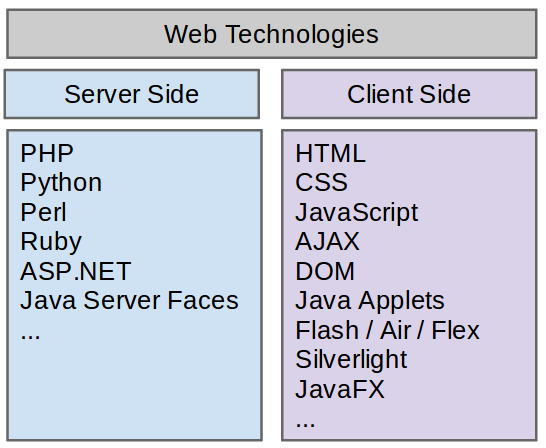
\includegraphics[width=0.61\textwidth]{./img/web-dev/web_technologies.png}
	\caption{Classification of web technologies}
	\label{fig:web-technologies}
\end{figure}

The client server architecture of the web also dictates the basic communication process.
The initial idea of the world wide web is that the client requests a static web page from a web server.
This static document contains styling information in form of HTML that can be interpreted by the client, the web browser, and is used to visualise the document.
For nearly every user interaction, the client sends a new request and the process repeats.
First with the introduction of Ajax by Jessie James Garret \autocite[]{ajax} it is initially possible to load data asynchronous and programatically from the server and to refresh the current page partially.
Ajax is a client side technology hence it allows the client to send a request and process its result asynchronously.
Usually Ajax works tightly together with JavaScript.

A pure server-side application uses a programming language like PHP, Perl or Ruby to dynamically generate a HTML document that is send to the client.
The client still just has to interpret and visualise static HTML documents.
The total application and business logic is handled by the server and every click on the page forces a reload of the total page.
All these points are disadvantageous when trying to integrate server driven web applications into a native Swing GUI.
Refreshing the whole application after every user interaction is in high contrast with the partial refresh of native desktop applications and needs to be avoided for a uniform user experience.
Current web frameworks admittedly offer ways to avoid this but only by using client side scripting and Ajax.
Ruby on Rails is a good example for that.
Although Ruby is a server side programming language and Rails a server side web framework, it brings support for prototype.js which is a JavaScript framework. Thus it possible to write dynamic and user friendly web applications that can be highly interactive.

Another even more important issue is, that always an additional web server is required, which is responsible for data management, application logic and session management which makes the interaction with the navigator GUI more difficult.
Just to give an example: How can the navigator be informed about data changes made in the web application? Furthermore, the most server side frameworks are intended to built full stack applications which means that they are also facilitate the creation of data models, persistence, authentication and son on.
This doesn't really match the situation, since those functionality is already implemented in the cids server respectively the new cids RESTful API which always provides a well defined interface for the client.

As already mentioned, rich user experience and interaction possibilities can only be implemented with client side technologies. Therefore it is inevitable to concentrate on client side technologies when developing web applications that shall be integrated into the navigator.

For a long, time significant differences in the user interaction of web applications and native desktop applications exist.
This is the reason why technologies like Adobe Flash or Java Applets came up, coining a totally new kind of web application, that should leave the drawbacks behind. With the increasing support of modern web standards such as HTML 5 , CSS3 and JavaScript in browsers, this limitation of native web applications fades away more and more. What all those technologies have in common, is that they allow to build rich internet applications, that offer the same level of user experience than native web applications. The following chapter therefore outlines and compares the different technologies that are available for building rich internet applications.


\section{Rich Internet Applications}

\subsection{Definition and Characteristics}

The term Rich Internet Application (RIA) was firstly introduced by Jeremy Allaire.
In \autocite[]{allaire_ria} he describes important characteristics of rich internet applications such as a powerful and extensible model for interactivity and using web and data services provided by application serves.
The term RIA is not standardized and there exist various definitions often with only a slight difference.


Bozzon et al state that RIAs are  \enquote{[...] a variant of Web-based systems providing sophisticated interfaces for representing complex processes and data, minimizing client-server data transfers and moving the interaction and presentation layers from the server to the client.} \autocite[]{ria-definition-1}
 
A good discussion on the various definitions can be found at \autocite[]{ria-state-of-the-art}.
They conclude that there are two parts that distinguishes RIA from "normal" web applications, a technical part and the user experience.
The technical differences are first and foremost the asynchronous data exchange with the server and the shift of application logic to the client.
The second part comprises the fact, that RIA's look and behave more like native desktop applications, in fact they have a richer user interaction and can be used on and offline.
 
\subsection{Technologies}

There are two groups of technologies with that rich internet applications can be build and that have evolved with the progress of client side web development technologies.
Bozzon et al \autocite{ria-classification-1} defines 4 categories of RIA technologies,scripting-based, plugin-based (Flash, Silverlight), browser-based (XUL, XAML) and web-based desktop technologies (Java Web Start).
A similar categorization can also be found in \autocite{ria-classification-2}.
The definition of web-based desktop technologies like Java WebStart as a RIA technology should be called into question.
Such applications are normal desktop applications, in case of Java Web Start Swing applications that are not executed in the browser an require a special runtime environment.
They merely use the web as deployment mechanism but can not be regarded as web applications.
Browser based RIA are more seldom which may be caused in the fact that they only run in a specific browser.
Both, browser based and web-based desktop technolgies,  are not suited for building web applications that can be used in the Swing based navigator GUI and as normal web application.

The more interesting types are plugin-based and sripting-based RIA's.
Plugin-based RIA's, as the name suggest, need a special and often vendor specific browser plugin or runtime environment.
Prominent candidates are Adobe Flash, Adobe Air, Microsoft Silverlight and JavaFX.
In \autocite[]{ria-comp-1} and \autocite[]{ria-comp-2} a good comparison of the most prominent plugin based RIA technologies can be found.

There are many issues with plugin based RIA's platforms.
The most important one is, that always an additional browser plugin is needed.
This limits the accessibility of web application and is contradictionary with the easy and wide spread acessibility of web applications.
Depending on the Platform it can happen that no plugin for every browser or operating system is available.
And even if there is a corresponding plugin available, it can not be guaranteed that the plugin is installed.
A good example for this are mobile devices.
There is no support for Flash on any iOS device.
In \autocite[]{jobs-thoughts-on-flash} Steve Jobs explain the reasons for this.
Some of the reason he mention, can also be transferred to other plugin based RIA platforms.
For example Jobs criticized that Flash \enquote{[...] has not performed well on mobile devices} \autocite[]{jobs-thoughts-on-flash}.
This issue belongs to all plugin based RIA platforms and and is not strictly limited to mobile devices.
They need a long time to load and initialize the application.
In addition, there is a considerably increased security risk with one or more browser plugins installed.
Flash in particular is well known for its security vulnerabilities.
Last but not least, most of the above mentioned platforms are not open an doesn't belong to a web standard.

Regarding all these issues and the latest improvements in web standards such as HTML5, CSS3 and JavaScript it is not surprising that the stake of web applications that use a plugin based RIA platform has decreased rapidly in the last years.
Figure \ref{fig:flash_usage} depicts the current usage of Flash and Silverlight and gives a back sight for the last three years.
From special interest is the decreasing stake of Adobe Flash, hence it is the most prominent and disseminated plugin based RIA technology.

\begin{figure}
	\centering 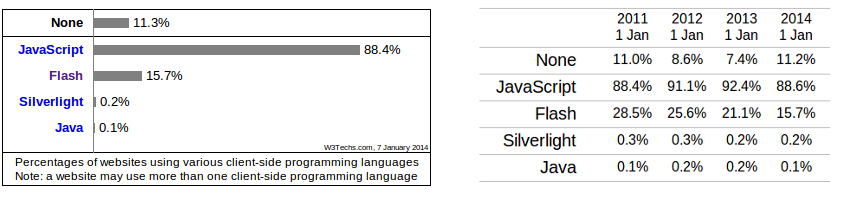
\includegraphics[width=1.0\textwidth]{./img/web-dev/flash_usage.png}
	\caption{usage client side web technologies \autocite[]{ria_flash-usage}}
	\label{fig:flash_usage}
\end{figure}

The last group of RIA's are solely implemented with web standards such as HTML5, CSS and JavaScript.
AJAX and JavaScript are the most important technologies for building web applications with a rich user interface in fact AJAX fundamentally changes the way the client communicates with the server.
The crucial advantage is that no special plugin or runtime environment is required. 
Scripting-based RIA's work in all standard conform web browser and on all devices.
This ensures that they have the same accessibility like normal web applications. For the sake of completeness it is important to note that it is possible in the most browser to disable the execution of JavaScript. But the pervasive and wide spread usage nowadays. A investigation in 2013 of Yahoo regrading this topic \autocite{web-dev:js-disabled}, claims that the maximum rate measured of users with disabled JavaScript support is roughly 2 percent. Regarding those facts, it seems that this argument can be neglected.

The immense improvements in the last years regarding new standards like HTML 5, CSS3 and JavaScript remedy a lot of the till then valid drawbacks of scripting based RIA's.
Just to give an example: Although they totally rely on standardized technologies, there are many differences how these standards are implemented in the different browsers, why it was often necessary to write browser depended code.
The principal issue still exists today, but owing to the presence of frameworks that abstract from the underlying browser those problems are avoided in the most cases.
Additionally, the rapid performance improvements of JavaScript engines in the last years, remedy the performance problem of pure script-based RIA's.
Another problem of script-based applications is, that they didn't have the same level of interaction richness.
But also this changed with the progresses that are achieved with JavaScript.
If we regard web applications like Google Mail, Facebook and Twitter just to name a few, it is clear that it is possible to write rich web applications solely with web standards and that behave and act like native desktop applications.
Upcoming technologies like local storage and client side data bases will even allow to develop web applications that can also be used without a connection to the internet.
Web Sockets will allow a bi-directional communication between the server and the client that can also be originated from the server and Web Workers will extend JavaScript with an asynchronous execution model.
Summing up, scripting based RIA's seems to be the most suitable approach for building web applications that can be integrated into the navigator. 
They offer a fairly good level of interactivity and the simple architecture will not additionally complicate the data exchange with the navigator. 

As already mentioned there are many efforts in building JavaScript frameworks and libraries that shall facilitate the development of rich JavaScript and HTML5 based web applications.
In the last year, a new emerging trend in that sector are frameworks that use the MVC pattern to structure the code, keep it maintainable and increase the development productivity.
This stands in contrast to the more matured frameworks like JQuery, YUI and Prototype which rather focuses on hiding browser specific implementation details and the DOM.
A detailed comparison of the actual existing JavaScript MVC is given in chapter \ref{chap:detail_comparison}.
The next chapter however, shall give a more conceptual overview over these new kind of frameworks.
 
\section{JavaScript MVC-Frameworks}

Modern JavaScript Frameworks like AngularJS, Ember and Knockout try to structure the code by using architectural patterns like MVC.
In order of doing this, they achieve a separation of presentation logic, business logic and presentation state.
Furthermore this seperation of concerns help developers to understand the framework much faster and get more comfortable with the it hence the used patterns provides them with a well known mental model.
Unfortunately not all frameworks use the classical MVC pattern as it is defined in \autocite[]{smalltalk_mvc}.
Some of them use slightly variants of this pattern like MVVM (Model-View-ViewModel or MVP (Model View Presenter).
Knockout for example uses the MVVM pattern to enable a loose coupling of the domain model and the view (cf.
\autocite{heise_knockout}).
 
The usage of the different pattern variations often lead to discussions of the various advantages and disadvantages of the used pattern and shifted the focus away from the frameworks itself.
But in fact all of the used patterns basically entail the same advantages, an Angular developer introduced the term MVW.
In he argues \enquote{Having said, I'd rather see developers build kick-ass apps that are well-designed and follow separation of concerns, than see them waste time arguing about MV* nonsense.
And for this reason, I hereby declare AngularJS to be MVW framework - Model-View-Whatever.
Where Whatever stands for "whatever works for you".} \autocite[]{anguler_mvw}.
This opinion finds more and more acceptance.

Another important feature that can be seen as a key concept of the new frameworks is automatic (two way) data binding between the model and the view.
This means that it is possible to bind UI elements like text, or input fields to properties of the correlating model.
Changes in the UI, for example user input, is automatically reflected to the model property, and programmatically changing the property updates the user interface.Figure \ref{fig:data-binding} demonstrates this.
This is an immense advancement in contrast to more ancient frameworks in fact the developer isn't responsible to write and test code for that purpose by hand or need to ensure manually that changes are reflected.
While there are multiple ways to achieve this, there are mainly two different approaches how the two way data binding is implemented.
A good and detailed examination of those implementations can be found in \autocite[]{binding_comparison}.
One approach is to use special JavaScript objects on the model site that are able to notify observers (the view) about changes.
This approach is used for example by EmberJS and Knockout.
The second approach allows to bind directly to plain old JavaScript objects.
Hence at the current JavaScript version it is not possible to get notified about changes of an objects value, a different approach is needed to detect changes.
The technique used there is periodically checking if any of the bound JavaScript objects has changed and updating the view for every changed object.
This process is often called Dirty Checking.
The two approaches have some fundamental consequences that are discussed into more detail in chapter \ref{chap:detail_comparison}

\begin{figure}
	\centering 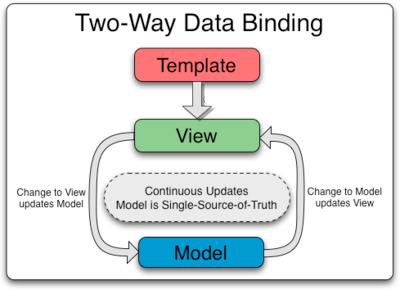
\includegraphics[width=0.61\textwidth]{./img/web-dev/data-binding.png}
	\caption{Two Way Data Binding \autocite{ng-binding}}
	\label{fig:data-binding}
\end{figure}

Very closely related to the two way data binding feature is the usage of template engines in modern JavScript MVC frameworks.
Templates support the developer in separating style and design from application and business logic.
Furthermore they make it unnecessary to programmatically generate html markup.
The template consists of html markup and some further place holders or variables where the final data gets inserted.

The template engines differ in the possibilities to integrate logic inside the templates.
Some allow full and arbitrary JavaScript logic, other a small set of constructs offered by the template engine itself, like loops, conditionals or partials.
The latter approach is the one that is mostly used, hence using arbitrary JavaScript in the templates is contrast with the initial idea of separating html markup and application logic.

Shifting the application logic to the client and only fetching data from the client creates also some new problems.
Hence the total application is loaded with the first request, no entries are added to the browsers history during the usage of the web application.
This destroys the browsers history and with it important functions like using the back and forward button or bookmarking certain states of the application.
This problem leads us the next core component that most of the modern frameworks provide, the routing mechanism.
Routing means that the different states of the application are mapped into an URL that can be used for the browsers history.
The mostly used approach nowadays is, to use the \enquote{\#} fragment identifier of the URL (cf. \autocite{spi_manifesto}).
The fragment identifier usually refers to an HTML element id or a named anchor in the current page and allows to automatically scroll to the position of that HTML element.
Current JavaScript frameworks use the fragment identifier to track the state of the application and the router components are responsible for turning the fragment identifier part of the URL to the right application state.

\begin{figure}
	\centering 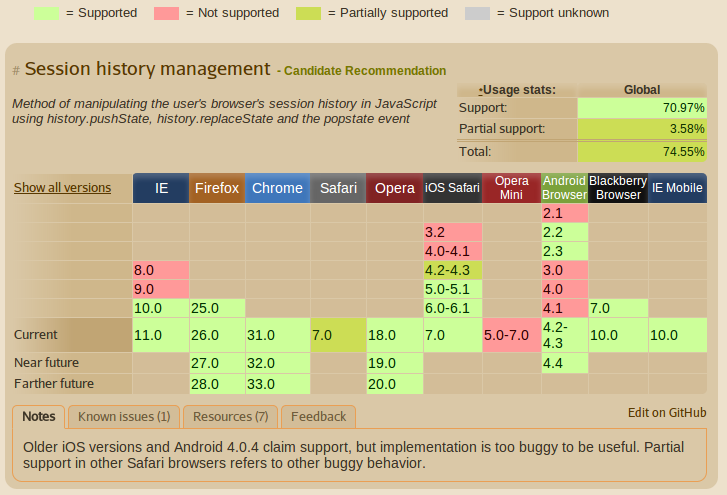
\includegraphics[width=0.8\textwidth]{./img/web-dev/usage_history_api.png}
	\caption{Browser Support History API \autocite{can_i_use}}
	\label{fig:usage_history_api}
\end{figure}

Using the fragment identifier for tracking application state is highly controversial.
There are a lot of blog posts and comments that discusses this approach (cf.
\autocite[]{hashbang_urls_1},\autocite[]{hashbang_urls_2},\autocite[]{hashbang_urls_3}).
To put the discussion in a nutshell the main arguments against this approach are, that it changes the target of the url, hence the fragment identifier is not send to the server, and only clients with JavaScript enabled can interpret these kind of URLs.
Using hash-bang URLs was the only possibility for tracking state in client side JavaScript applications.
Fortunately the upcoming HTML 5 standard contains a new part, the History API \autocite[]{w3c-history-api}, that allows the browser to modify the current URL and the browser history programmatically.
The History API offers a new way for tracking application state without using hash-bang URLs and the related drawbacks.
Hence most browsers already support the History API (see also figure \ref{fig:usage_history_api}) it is just a matter of time till this feature replace hash-bang URLs in the frameworks.
Angular for example already offers the possibility to already use the History API (cf.
\autocite[]{angular_location}).

\begin{figure}
	\centering 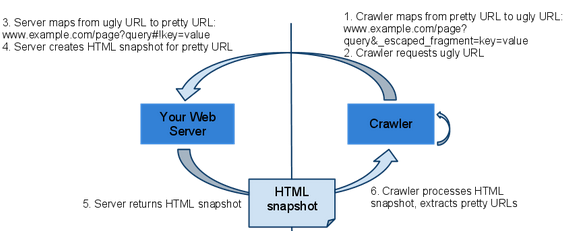
\includegraphics[width=1.0\textwidth]{./img/web-dev/google_crawling_hashbang.png}
	\caption{Google crawling AJAX \autocite{google_AJAX_crawling}}
	\label{fig:google_crawling_ajax}
\end{figure}

Another problem that comes up using JavaScript driven web applications is that they can't be analysed from search engines as easily as server centric web applications because the initial page request doesn't return a HTML document that contains the important content directly.
But also for this drawback certain technologies exists, that remedy this disadvantage.
The first on was announced from Google in 2009.
In \autocite[]{google_AJAX_crawling} they announce a method to crawl hash-bang URLs.
The main idea is that the crawler maps the hash-bang URL into an normal URL that contains the fragment identifier.
Figure \ref{fig:google_crawling_ajax} depicts the idea.
Important to note is that the web server needs to deliver a custom and search engine optimized HTML document for the URL.
This is what all approaches have in common.
An other upcoming approach, that gets more and more popular, is to use a headless web browser like PhantomJS on server side that is able to parse the web application like a normal browser and can output the normal HTML markup to the search bot.